\section{Latent demand recovery và kiểm soát imputation}

\subsection{Kết quả recovery tổng quan}

Bảng sau tóm tắt kết quả recovery. Recovered demand tăng khoảng 10.68\% so với observed sales. Về business, con số này có thể hiểu là phần demand tiềm ẩn mà observed sales không phản ánh đầy đủ do stockout.


\begin{table}[H]
\centering
\caption{Tóm tắt latent demand recovery}
\label{tab:long-recovery-summary}
\resizebox{\linewidth}{!}{%
\begin{tabular}{ll}
\toprule
Metric & Value \\
\midrule
Observed sales & 482697.09375 \\
Recovered latent demand & 534270.1875 \\
Recovered lost demand & 51572.875 \\
Recovered lift over observed & 0.10684314370155334 \\
Stockout row rate & 0.24652109375 \\
Recovery method & expanding-window weekly recovery \\
Imputation calibration factor & 1.1297638401922185 \\
Lost demand cap quantile & q90 of calibrated positive lost demand \\
Lost demand cap value & 0.06627678871154785 \\
Warmup days kept observed & 14 \\
Recovery block days & 7 \\
Recovery blocks & 9 \\
Final recovery train rows & 400000 \\
Recovery train source & past non-stockout rows only for train blocks; train-period non-stockout rows for validation/test \\
Final recovery train end & 2024-06-10 23:00:00 \\
Validation start & 2024-06-11 00:00:00 \\
Test start & 2024-06-18 00:00:00 \\
\bottomrule
\end{tabular}
}
\end{table}



\begin{figure}[H]
    \centering
    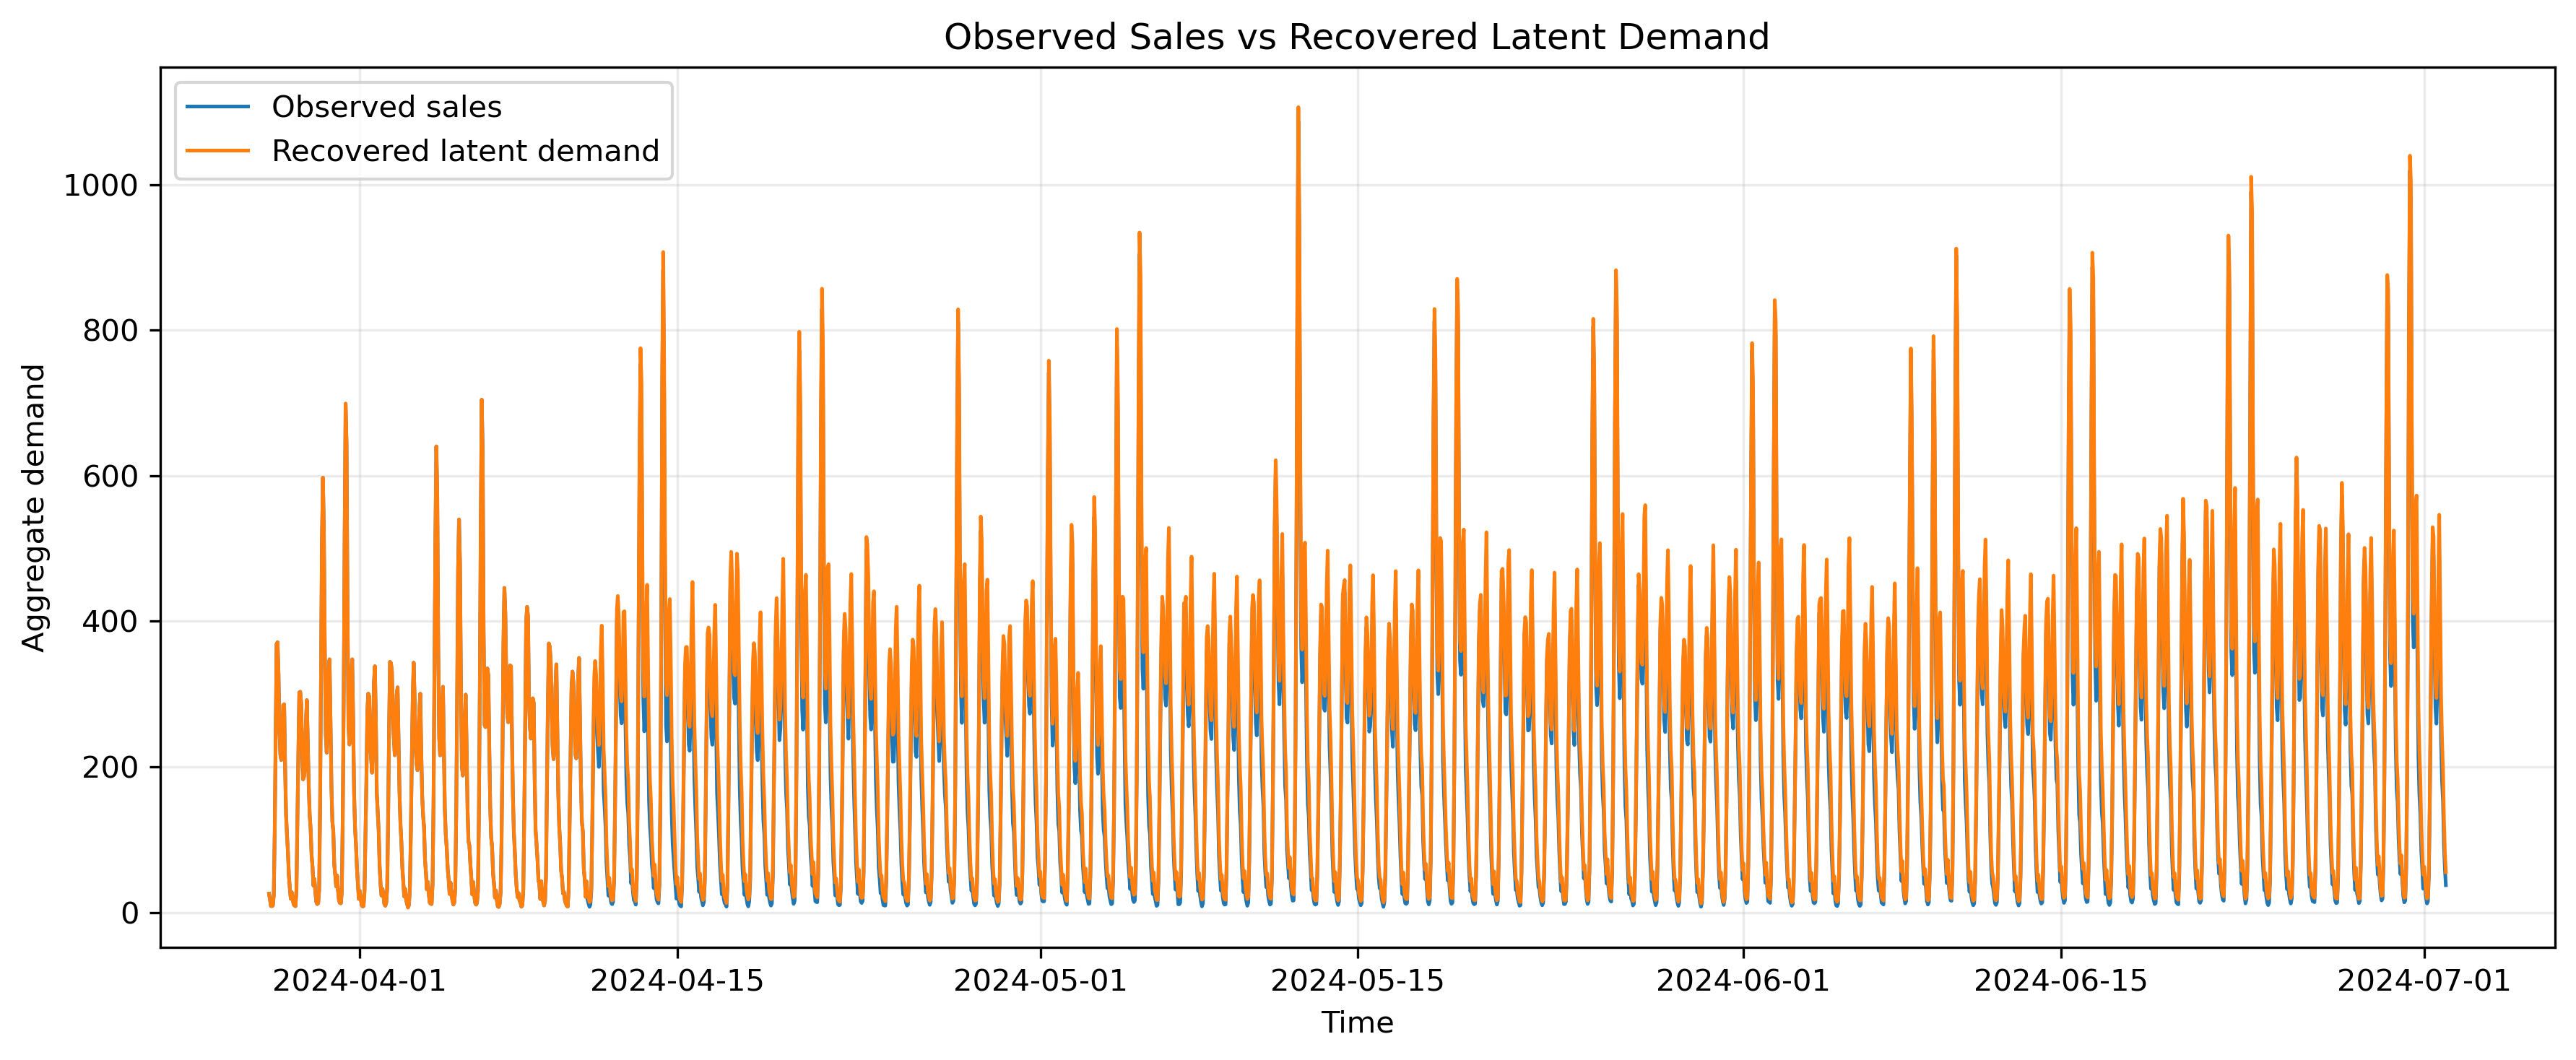
\includegraphics[width=0.92\linewidth]{figures/owner_observed_vs_recovered_demand.png}
    \caption{Observed sales và recovered demand theo thời gian.}
    \label{fig:long-observed-recovered}
\end{figure}


\subsection{Uplift do imputation}

Vì recovered demand không phải ground truth thật, báo cáo không dùng imputation một cách mù quáng. Uplift được kiểm tra ở nhiều cấp: tổng dataset, từng ngày và từng series. Nếu uplift quá lớn hoặc tập trung ở một số series, kết quả forecast sẽ phụ thuộc quá mạnh vào imputation.


\begin{table}[H]
\centering
\caption{Tổng mức uplift do imputation}
\label{tab:long-uplift}
\resizebox{0.86\linewidth}{!}{%
\begin{tabular}{ll}
\toprule
Metric & Value \\
\midrule
Observed sales & 482,697 \\
Recovered demand & 534,270 \\
Recovered lost demand & 51,573 \\
Recovered lift over observed & 0.1068 \\
Raw calibrated lost demand before cap & 65,368 \\
Cap retained share of raw lost demand & 0.7890 \\
Stockout row share & 0.2465 \\
Recovered lost demand from stockout rows & 51,573 \\
Mean stockout uplift per stockout row & 0.0182 \\
\bottomrule
\end{tabular}
}
\end{table}



\begin{figure}[H]
    \centering
    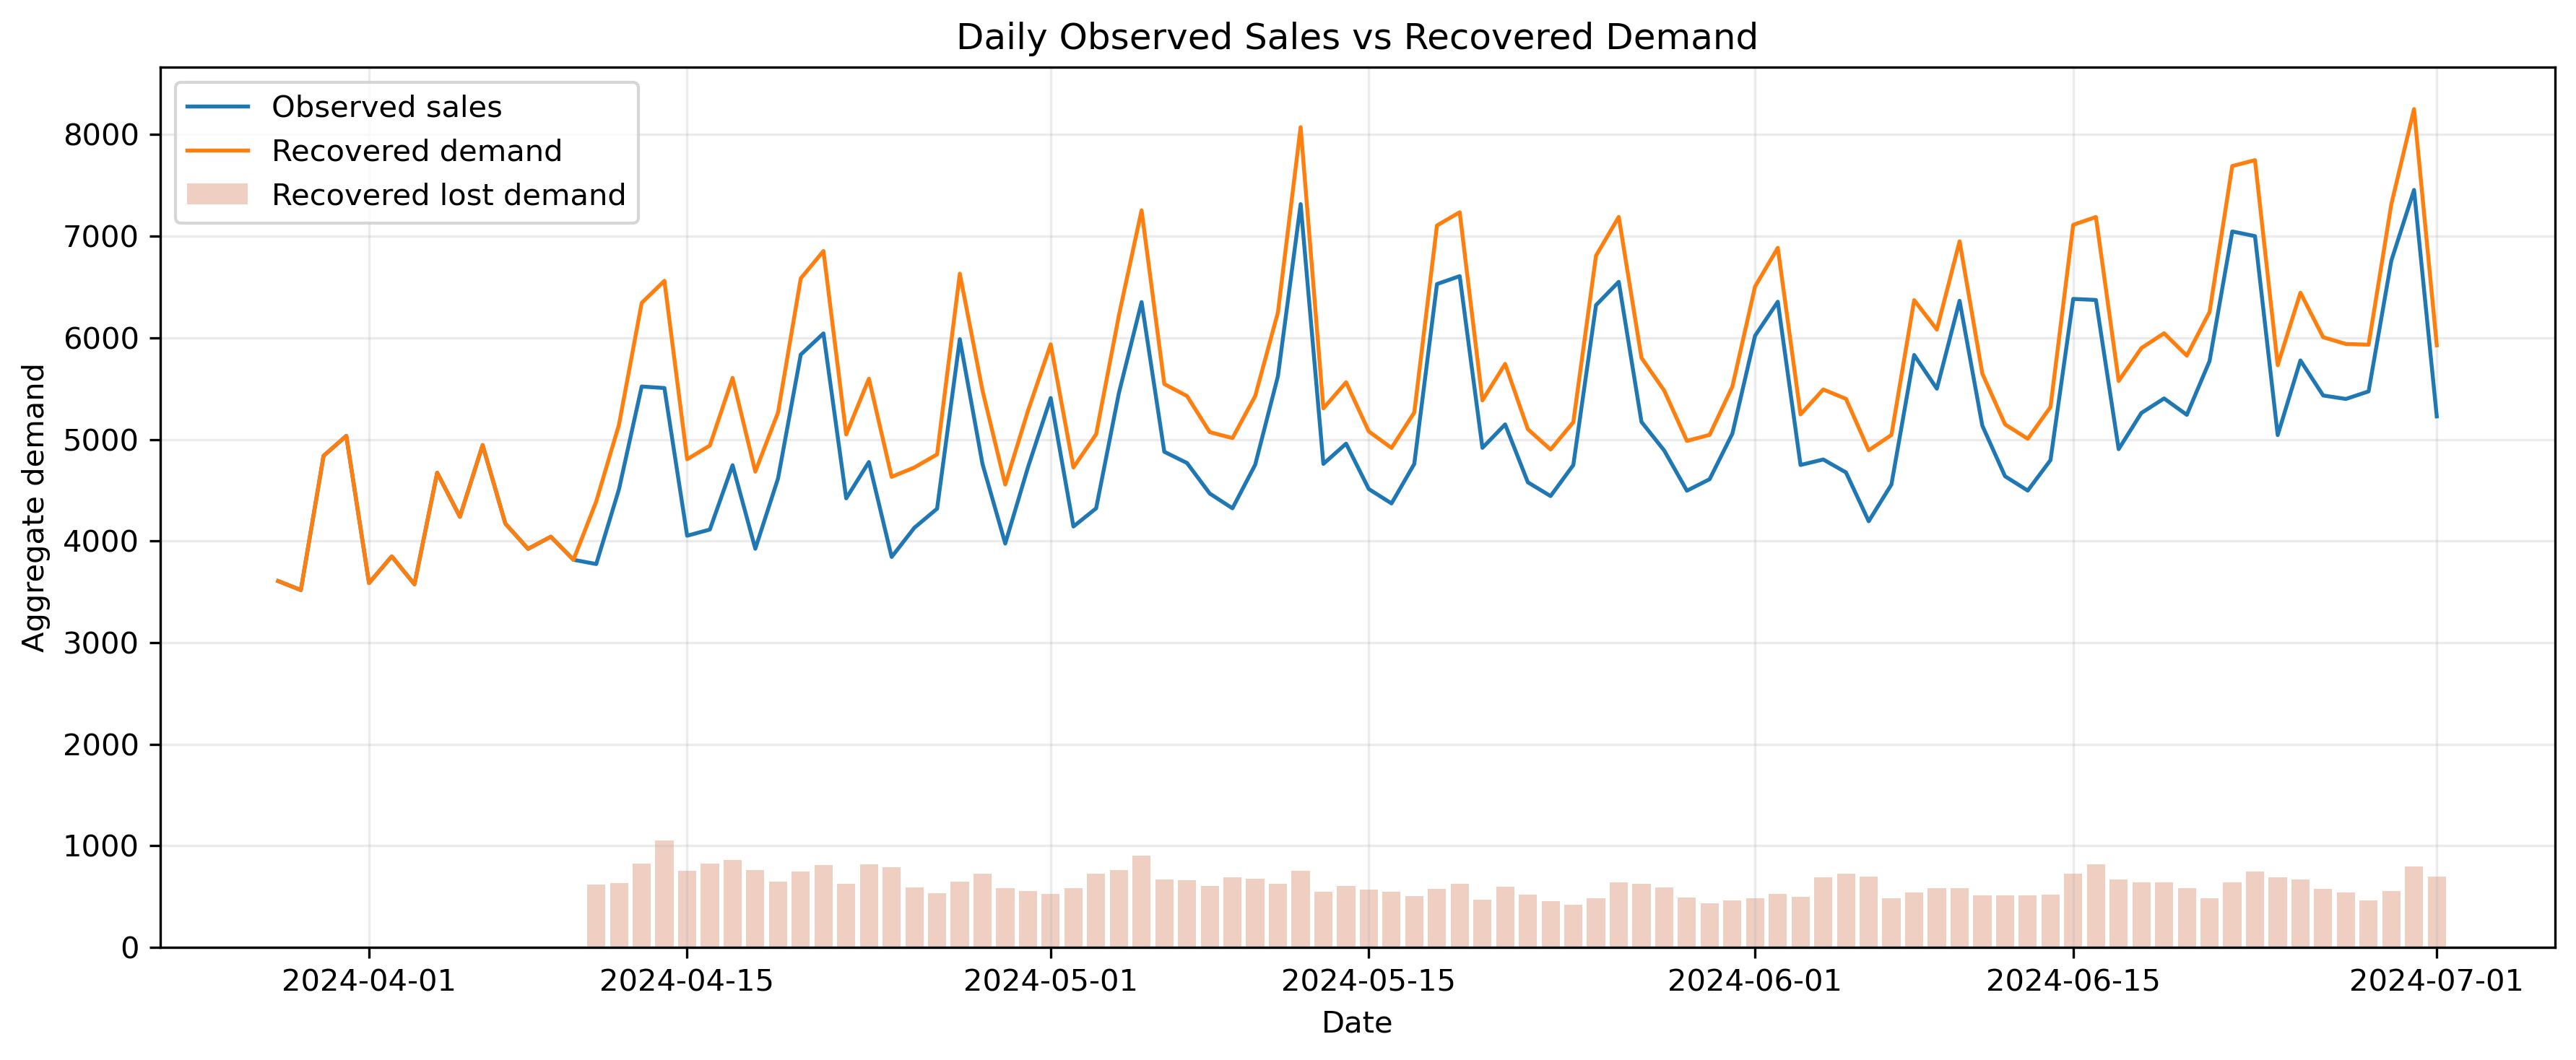
\includegraphics[width=0.92\linewidth]{figures/imputation_daily_uplift.png}
    \caption{Observed sales, recovered demand và recovered lost demand theo ngày.}
    \label{fig:long-daily-uplift}
\end{figure}


\subsection{Pseudo-stockout validation}

Pseudo-stockout validation lấy các dòng non-stockout trong validation period, giả sử chúng cần impute, rồi so sánh prediction của recovery model với observed sales thật. Row-level hourly validation có WAPE cao vì hourly sales rất thưa và nhiều giá trị nhỏ. Do đó, báo cáo bổ sung aggregate validation, phù hợp hơn với mục tiêu forecast daily demand.


\begin{table}[H]
\centering
\caption{Pseudo-stockout validation ở cấp row hourly}
\label{tab:long-pseudo-row}
\resizebox{0.86\linewidth}{!}{%
\begin{tabular}{ll}
\toprule
Metric & Value \\
\midrule
Validation rows & 300000 \\
Pseudo-stockout source & non-stockout rows from validation period \\
RMSE & 0.10030610859394073 \\
MAE & 0.05774029344320297 \\
WAPE & 1.0391554832458496 \\
sMAPE & 1.6277295807119518 \\
Mean prediction / actual ratio & 1.1315665245056152 \\
Mean error actual-minus-imputed & -0.007310444954782724 \\
\bottomrule
\end{tabular}
}
\end{table}



\begin{table}[H]
\centering
\caption{Pseudo-stockout validation ở các cấp aggregate}
\label{tab:long-pseudo-agg}
\resizebox{\linewidth}{!}{%
\begin{tabular}{lllllll}
\toprule
Validation level & RMSE & MAE & WAPE & sMAPE & Prediction / actual ratio & N \\
\midrule
Hourly aggregate & 42.5877 & 21.9068 & 0.2208 & 0.2237 & 1.1316 & 168 \\
Daily aggregate & 450.9920 & 416.6911 & 0.1750 & 0.1677 & 1.1316 & 7 \\
Series daily aggregate & 0.3245 & 0.2155 & 0.4384 & 0.6309 & 1.1316 & 33907 \\
\bottomrule
\end{tabular}
}
\end{table}


\subsection{Sensitivity theo cap}

Cap q90 được chọn như một điểm cân bằng. Cap q75 bảo thủ hơn nhưng có thể under-recover; q100 giữ toàn bộ raw lost demand nhưng dễ phụ thuộc mạnh vào outlier. Sensitivity giúp chứng minh kết luận không chỉ dựa trên một lựa chọn cap tùy tiện.


\begin{table}[H]
\centering
\caption{Sensitivity theo mức cap lost demand}
\label{tab:long-cap-sensitivity}
\resizebox{\linewidth}{!}{%
\begin{tabular}{llllll}
\toprule
Scenario & Cap value & Recovered demand & Recovered lost demand & Recovered lift over observed & Share of original recovered lost demand \\
\midrule
Cap lost-demand at q50 & 0.0151 & 505,963 & 23,266 & 0.0482 & 0.3559 \\
Cap lost-demand at q75 & 0.0369 & 523,781 & 41,084 & 0.0851 & 0.6285 \\
Cap lost-demand at q90 & 0.0663 & 534,270 & 51,573 & 0.1068 & 0.7890 \\
Cap lost-demand at q100 & 2.7508 & 548,064 & 65,368 & 0.1354 & 1.0000 \\
\bottomrule
\end{tabular}
}
\end{table}



\begin{figure}[H]
    \centering
    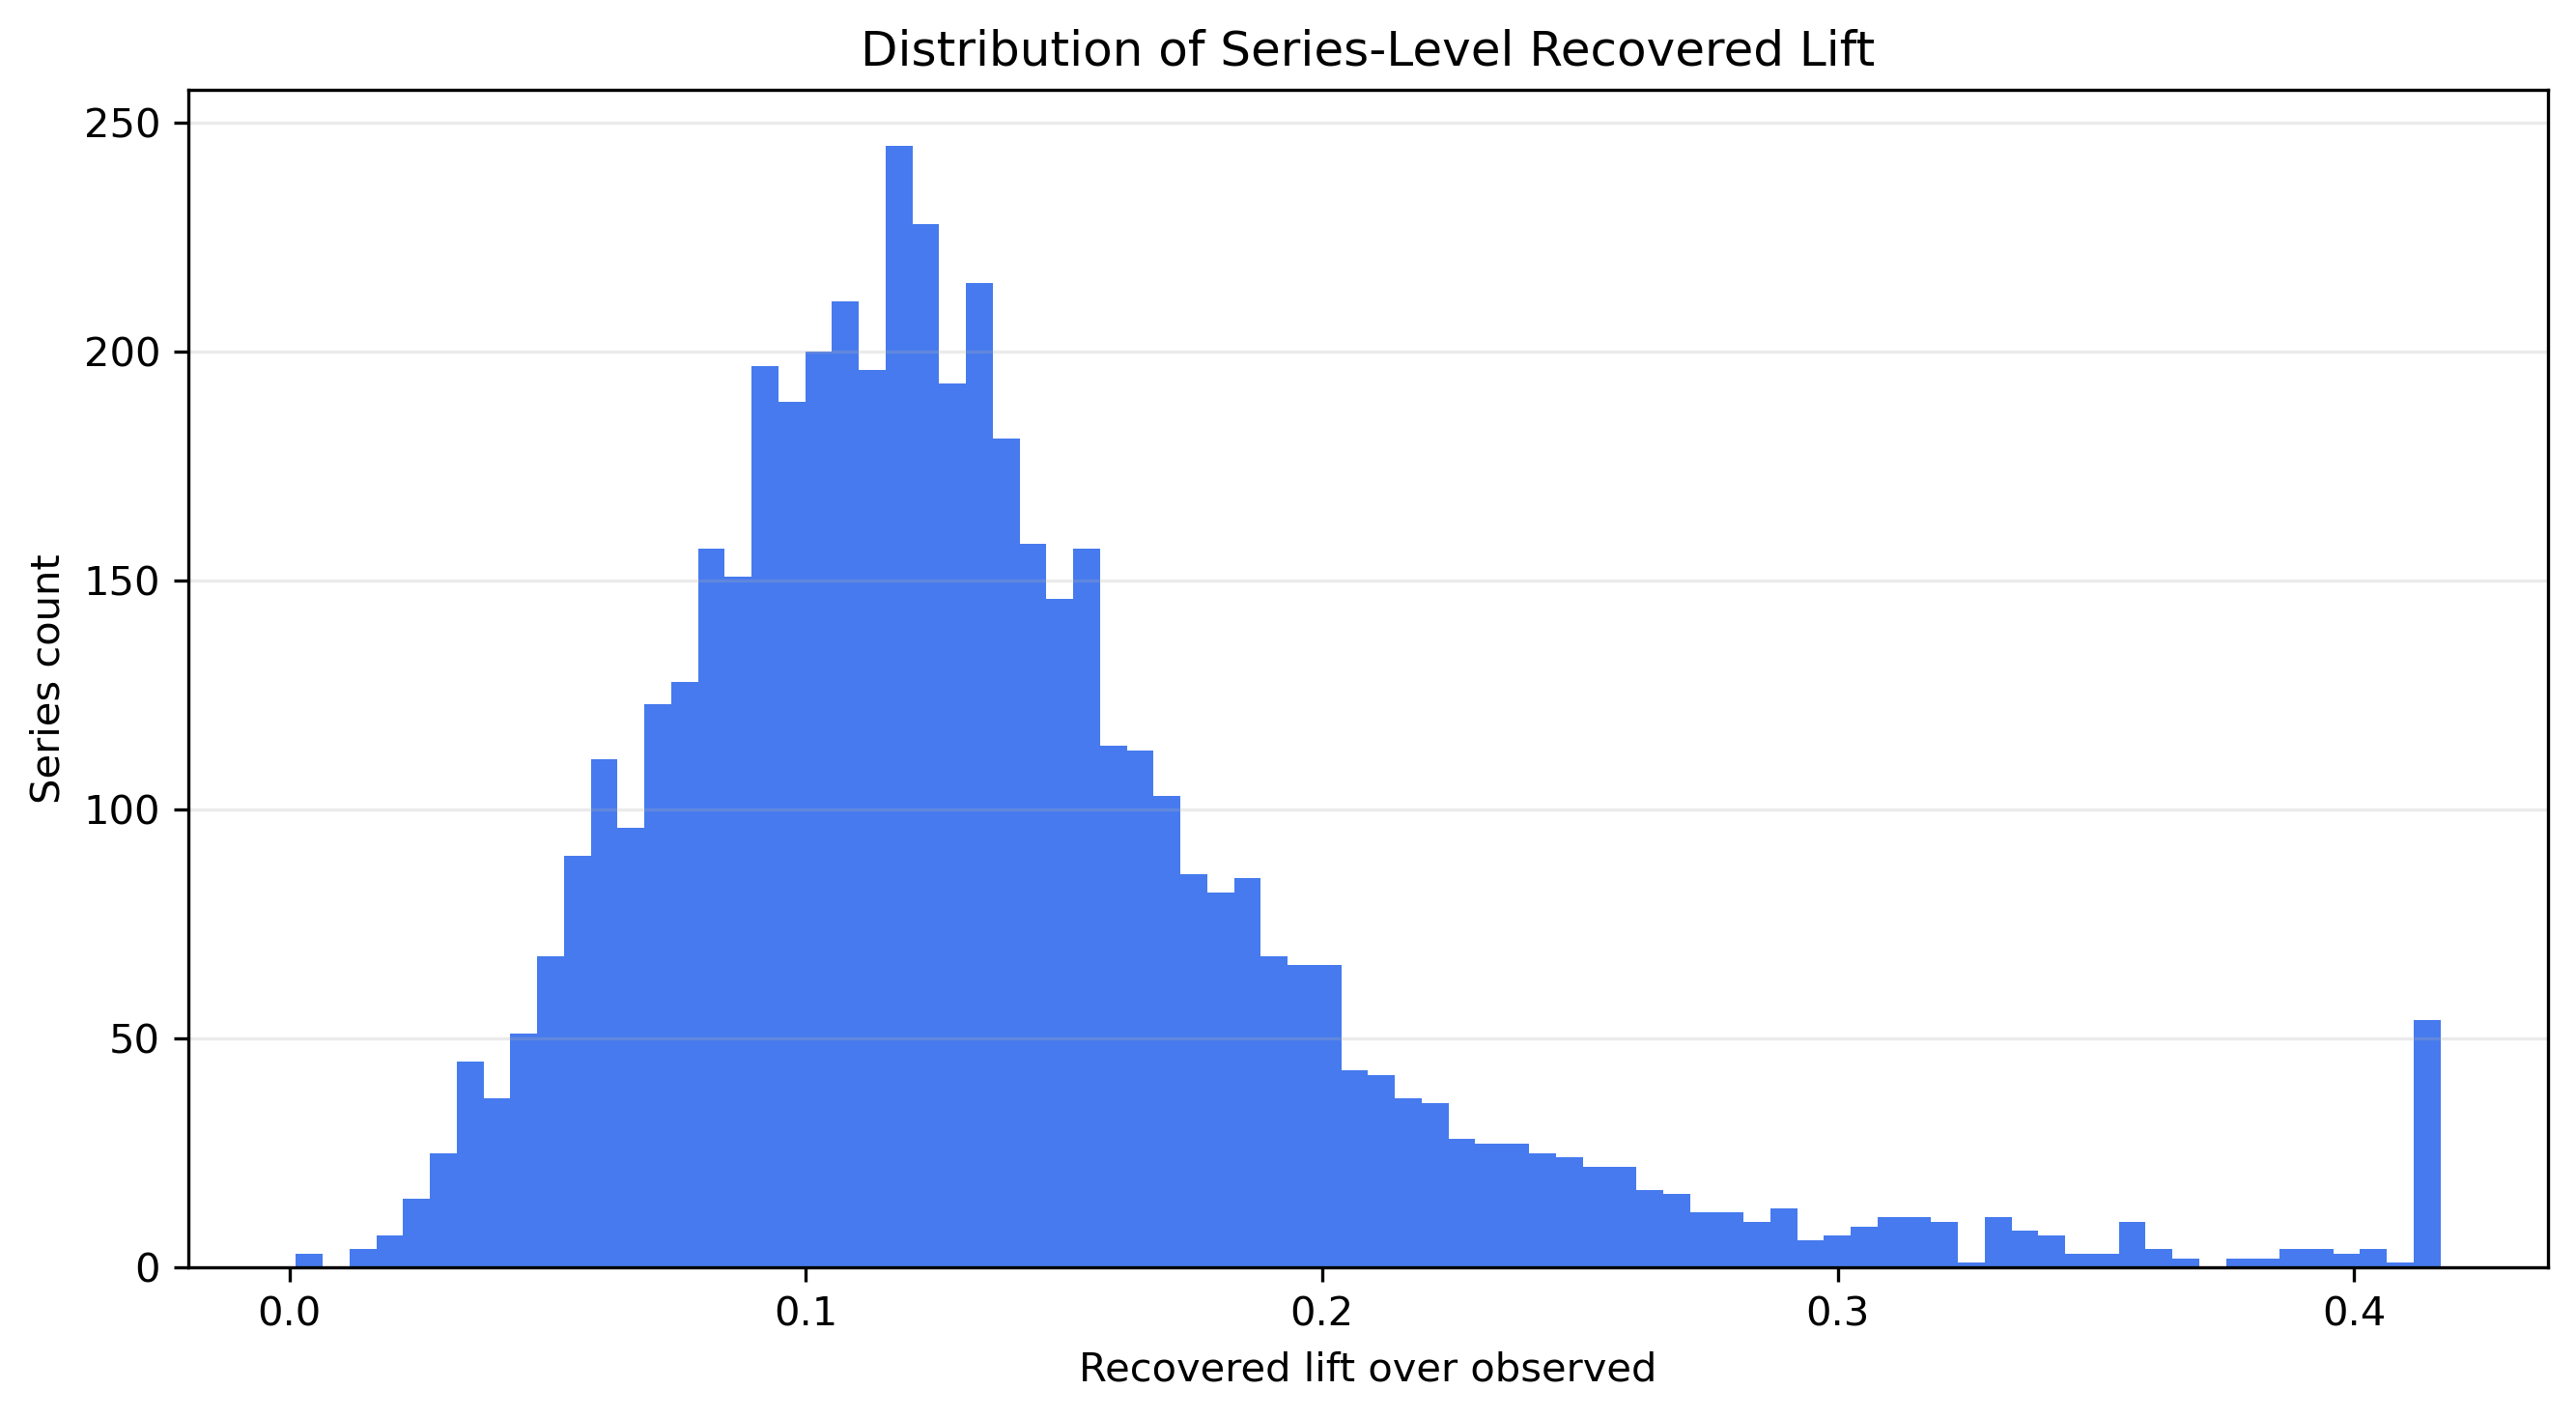
\includegraphics[width=0.78\linewidth]{figures/imputation_series_lift_distribution.png}
    \caption{Phân phối recovered lift ở cấp series.}
    \label{fig:long-lift-dist}
\end{figure}



\begin{figure}[H]
    \centering
    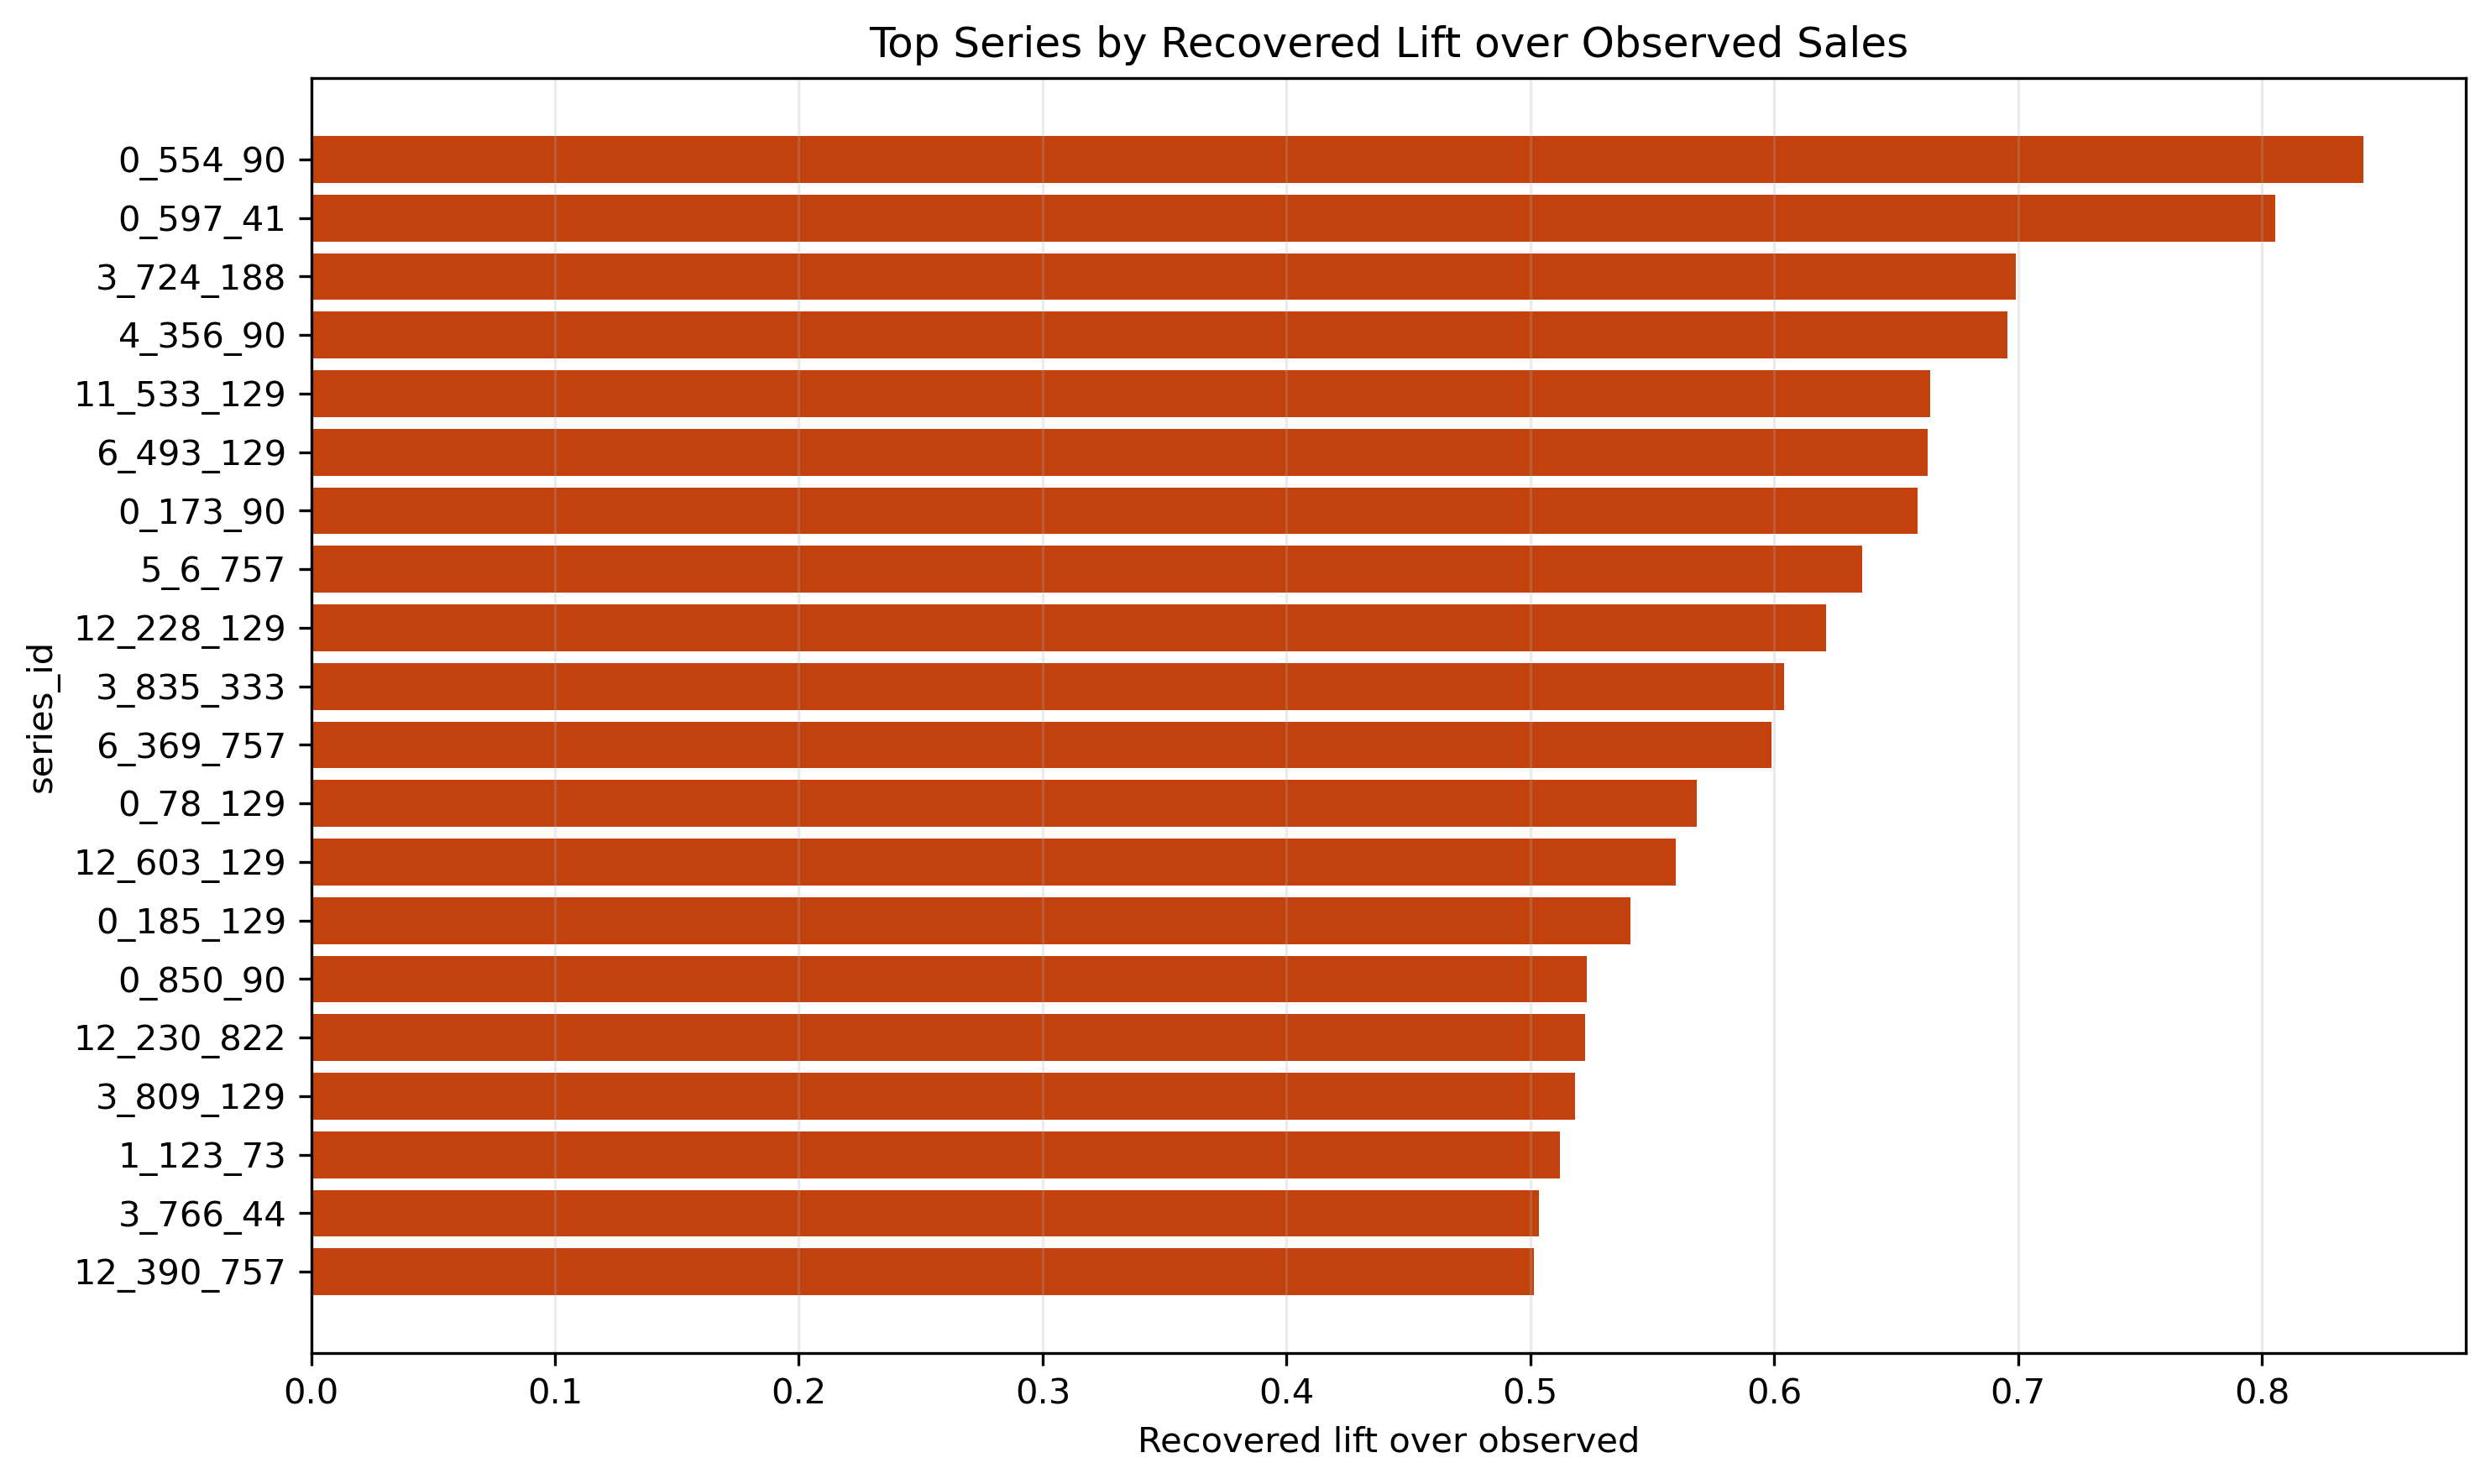
\includegraphics[width=0.78\linewidth]{figures/imputation_top_series_lift.png}
    \caption{Top series có lift cao nhất.}
    \label{fig:long-top-lift}
\end{figure}
